% This is the results section og the report on homework-2.
% Author(s) : Vivek Kumar / Victor Charpentier
% Last Updated : 04/03/2018
%%%%%%%%%%%%%%%%%%%%%%%%%%%
\section{Results and Discussion}
The first result we present is that of cross-validation performed on the split data to determine the best for each prediction. The total train data (obtained from {\ttfamily train.csv}) was divided randomly into a 50:50 split. The cross-validation score chosen for comparison was mean-squared-error (MSE). The results for each are displayed in table[]

\begin{table}[H]
\centering
	\begin{tabular}{|c|c|c|c|}
	\hline
	Method & GPA MSE & Grit MSE & Material Hardship MSE\\
	\hline
	RandomForestRegressor	&	0.221031	&	0.153470	&	0.015116	\\
	AdaBoostRegressor		&	0.250311	&	0.156094	&	0.017874	\\
	LassoLarsCV				&	0.232776	&		&		\\
	ElasticNet				&	0.379290	&		&		\\
	ExtraTreesRegressor		&	0.219626	&	0.162074	&	0.016035	\\
	MLPRegressor			&	157140	&	190226	&	305336	\\
	\hline
	\end{tabular}
	\caption{Mean-Squared-Error score for various methods obtained in cross-validation}
\end{table}
Using the best method the leaderboard scores were :
\begin{align*}
\mathrm{GPA \ Score \ :}  && \mathrm{Grit \ Score \ :}  && \mathrm{Material \ Hardship \ Score \ :}
\end{align*}
The bootstrapping was performed on the training data set to determine the minimum and maximum error obtained for each prediction. Here we have used RandomForestRegressor as the method for predicting the results. The results are plotted in the Figure [].

Further to understand, which features were most important the {\ttfamily mutual\_info\_regression} from {\ttfamily feature\_seclection} of sklearn was used. The plot shows the mutual information between each feature and the target prediction.
\begin{figure}[H]
\centering
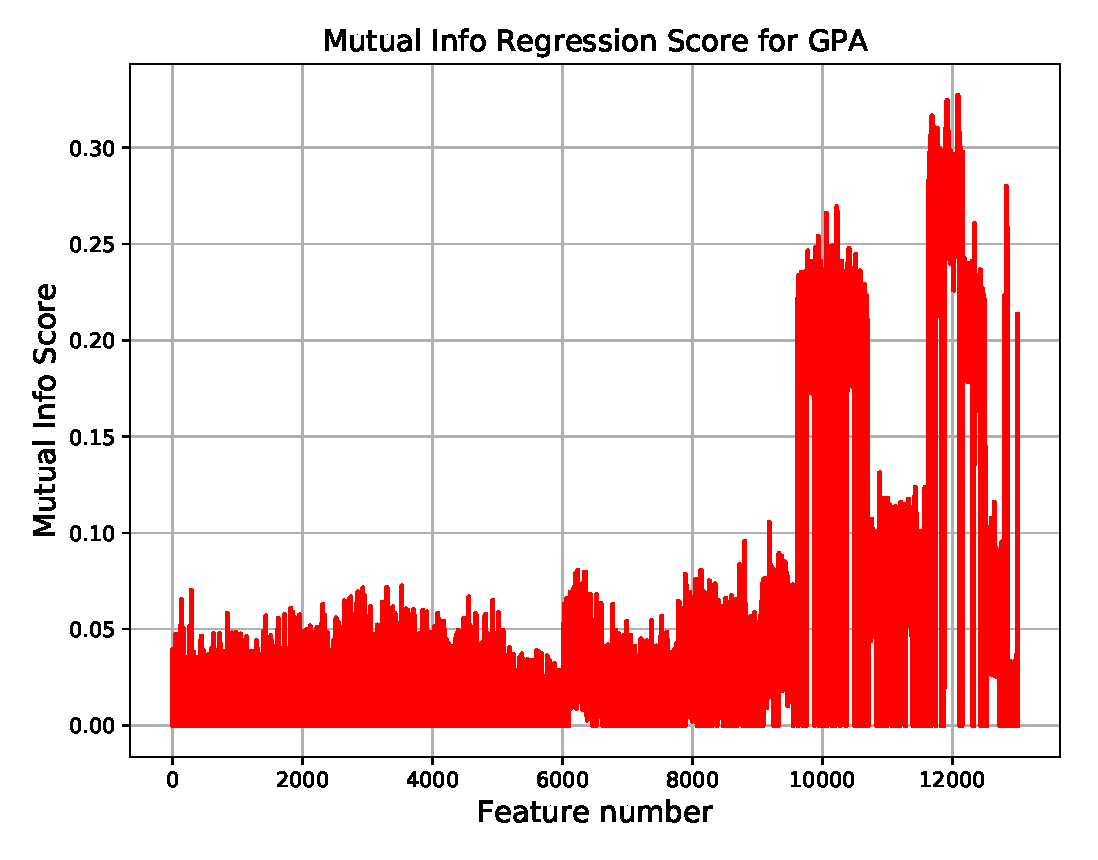
\includegraphics[width=0.49\textwidth]{feature_selection_gpa_scores}
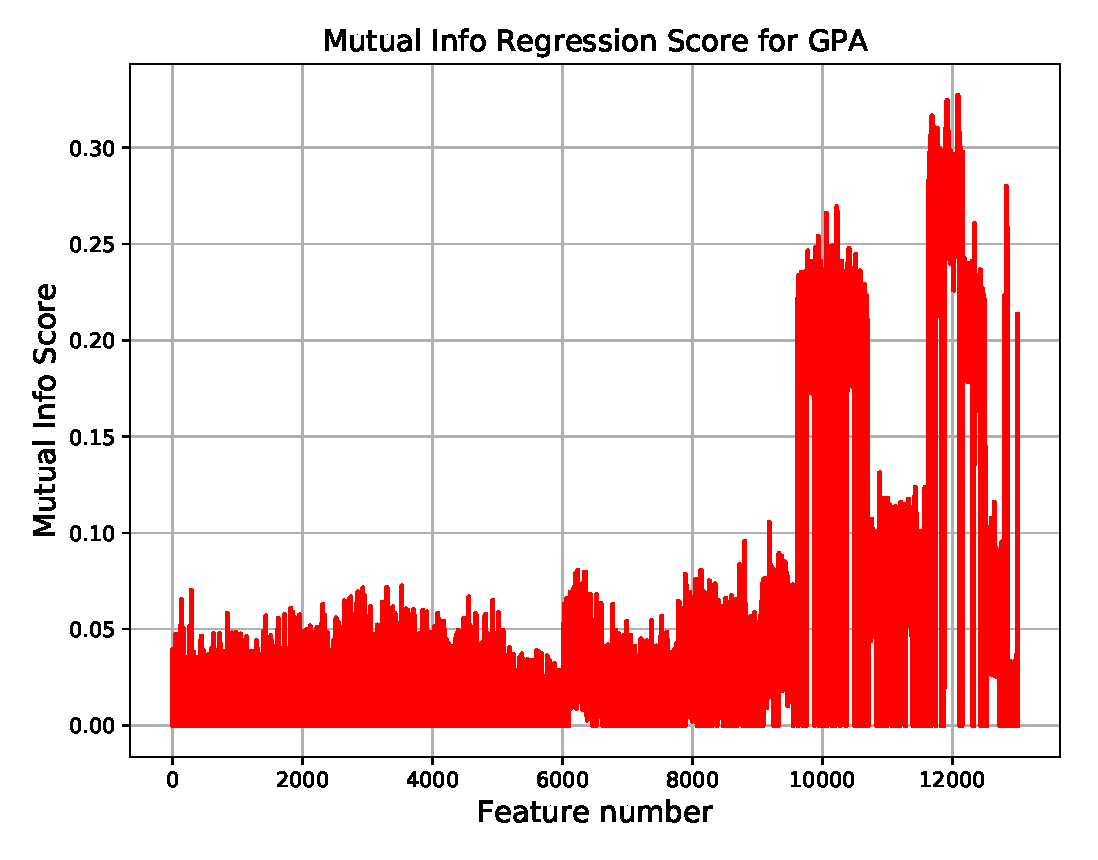
\includegraphics[width=0.49\textwidth]{feature_selection_gpa_scores}
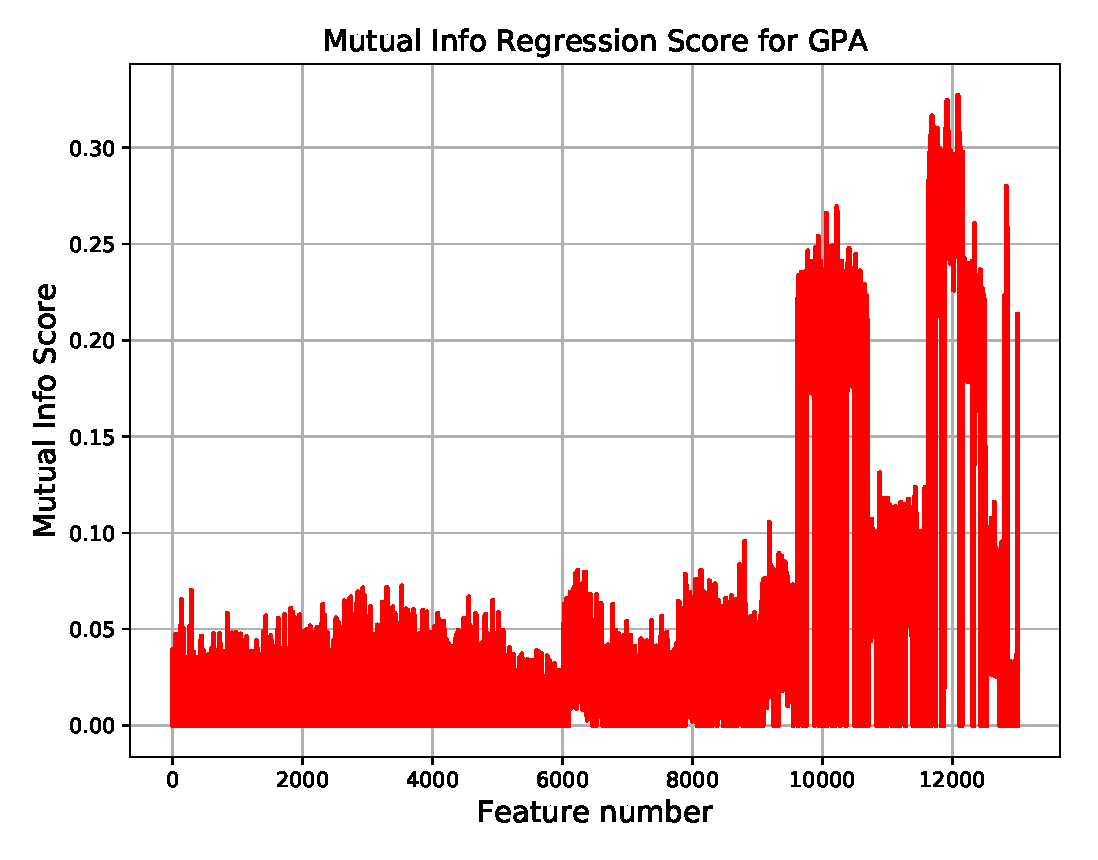
\includegraphics[width=0.49\textwidth]{feature_selection_gpa_scores}
\end{figure}

\begin{table}[H]
\centering
	\begin{tabular}{|c|c|c|c|}
	\hline
	Method & None & Mutual Info (k-best) & PCA(99\% variance)\\
	\hline
	RandomForestRegressor	&	0.221031	&	0.226496	&	0.015116	\\
	AdaBoostRegressor		&	0.250311	&	0.240569	&	0.017874	\\
	LassoLarsCV				&	0.232776	&	0.233773	&		\\
	ElasticNet				&	0.379290	&	0.245301	&		\\
	ExtraTreesRegressor		&	0.219626	&	0.223951	&	0.016035	\\
	MLPRegressor			&	157140	&	51837	&	305336	\\
	\hline
	\end{tabular}
	\caption{Mean-Squared-Error score for GPA with and without dimension reduction/ feature-selection}
\end{table}

We also employed the principal component analysis for dimension-reduction. Instead of showing the individual results we compare how the methods performed when various feature selection or dimension reduction techniques were employed.

